\documentclass[border=3pt,tikz]{standalone}
\usepackage{amsmath}
\usetikzlibrary{calc}
\usetikzlibrary{arrows.meta} % for arrow size
\begin{document}

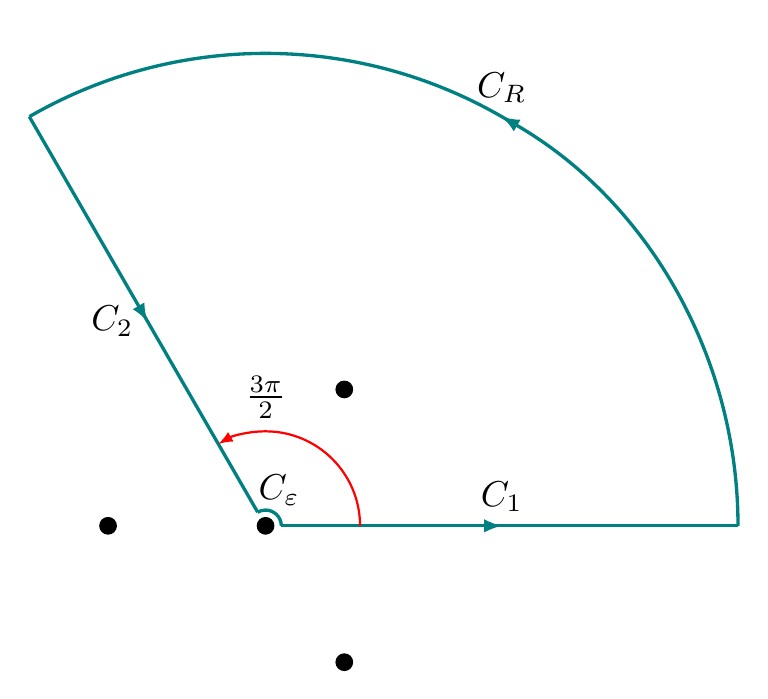
\begin{tikzpicture}[scale=2]
    \usetikzlibrary {arrows.meta}
    \usetikzlibrary {calc}
    
    \coordinate (O) at (0, 0);
    \coordinate (P1) at (0, 3);
    \coordinate (P2) at ({3*cos(60)}, {3*sin(60)});
    \coordinate (P3) at ({3*cos(120)}, {3*sin(120)});
    
    \draw[teal, very thick, -latex] (0.1, 0) -- (1.5, 0) node[above, black, scale=1.3] {$C_1$};
    \draw[teal, very thick] (1.4, 0) -- (3, 0);
    \draw[teal, very thick, -latex,] (3, 0) arc (0:60:3) node[black,above, scale=1.3] {$C_R$};
    \draw[teal, very thick,] ({3.0*cos(58)}, {3.0*sin(58)}) arc (58:120:3);
    \draw[teal, very thick, -latex] ( {3.0*cos(120)}, {3.0*sin(120)}) -- ({1.5*cos(120)}, {1.5*sin(120)}) node [left, black, scale=1.3] {$C_2$};
    \draw[teal, very thick] ({1.6*cos(120)}, {1.6*sin(120)}) -- ({0.1*cos(120)}, {0.1*sin(120)});
    
    \draw[teal, very thick] (0.1, 0) arc (0:120:0.1);
    
    \filldraw[black] (O) circle (1.5pt);
    \filldraw[black] ({cos(60)}, {sin(60)}) circle (1.5pt);
    \filldraw[black] ({cos(180)}, {sin(180)}) circle (1.5pt);
    \filldraw[black] ({cos(300)}, {sin(300)}) circle (1.5pt);
    
    \draw[red, thick, -latex] (0.6, 0) arc (0:120:0.6);
    \node[above, scale=1.3] at (0, 0.6) {$\frac{3\pi}{2}$};
    \node[above, scale=1.3] at ({0.1*cos(30)}, {0.1*sin(30)}) {$C_\varepsilon$};
    
    \end{tikzpicture}
\end{document}